
\begin{frame}
\frametitle{Administración del plan de riesgo}
Es el proceso de definir como realizar las actividades de gestión de riesgo del proyecto.

Se debe:
\begin{itemize}
    \item Planificación \textbf{cuidadosa} y bien definida mejora las probabilidades de
    triunfar en los 5 otros procesos de la administración del riesgo.
    \item Proceso que \textbf{comienza} cuando el proyecto es concebido.
\end{itemize}
\begin{columns}
	\begin{column}{0.6\textwidth}
	\end{column}
	\begin{column}{0.4\textwidth}
		\includegraphics[width=3cm]{img/random_img_1}
	\end{column}
\end{columns}
\end{frame}

%\subsection{Valores de entrada}
\begin{frame}
\frametitle{Administración del plan de riesgo}
\framesubtitle{Valores de entrada}

\begin{columns}
	\begin{column}{0.8\textwidth}
\begin{itemize}
    \item<1-> \textbf{Alcances} del proyecto.
    \item<2-> Plan de la administración de \textbf{costos}.
    \item<3-> Plan de administración de \textbf{tiempos}.
    \item<4-> Plan de administración de \textbf{Comunicaciones}.
    \item<5-> \textbf{Factores} del ambiente empresarial.
    \item<6-> Información organizacional de los \textbf{procesos}.
\end{itemize}
	\end{column}
	\begin{column}{0.2\textwidth}
		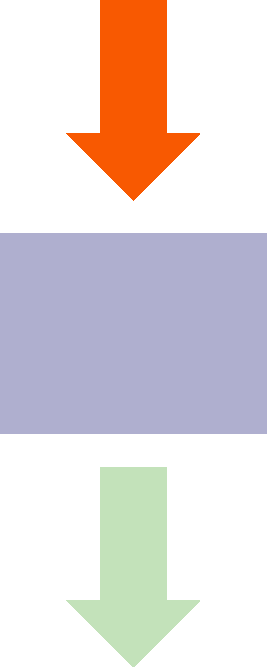
\includegraphics[width=2cm]{img/input}
	\end{column}
\end{columns}
\end{frame}

%\subsection{Técnicas y Herramientas}
\begin{frame}
\frametitle{Administración del plan de riesgo}
\framesubtitle{Técnicas y Herramientas}
\begin{columns}
	\begin{column}{0.8\textwidth}
\begin{itemize}
    \item \textbf{Reuniones} de análisis y elaboración del plan de administración de riesgo.
    \begin{itemize}
        \item<1-> Requieren de todos los \textbf{involucrados} del proyecto.
        \item<2-> Se busca definir las \textbf{actividades} para la administración del riesgo.
        \item<3-> Se calculan los \textbf{costos} respectivos.
        \item<4-> Revisiones de las \textbf{medidas} de contingencia.
        \item<5-> Asignación de \textbf{responsabilidades}.
        \item<6-> \textbf{Categorización} de riesgos por nivel, probabilidad, impacto, etc.
        \item<7-> Generación de \textbf{templates}.
    \end{itemize}
\end{itemize}
	\end{column}
	\begin{column}{0.2\textwidth}
		\includegraphics[width=2cm]{img/tools}
	\end{column}
\end{columns}
\end{frame}

%\subsection{Valores de Salida}
\begin{frame}
\frametitle{Administración del plan de riesgo}
\framesubtitle{Valores de Salida}
\begin{columns}
	\begin{column}{0.8\textwidth}
\begin{itemize}
    \item<1-> \textbf{Metodología}.
    \item<2-> \textbf{Roles} y responsabilidades.
    \item<3-> \textbf{Presupuesto}.
    \item<4-> Periodos de \textbf{evaluación}.
    \item<5-> \textbf{Categorías} de riesgos.
    \item<6-> \textbf{Definiciones} de probabilidad y impacto de los riesgos.
    \item<7-> Matriz de \textbf{probabilidad} e \textbf{Impacto}.
    \item<8-> \textbf{Tolerancia} de los stakeholders.
    \item<9-> \textbf{Formatos} de reporte.
    \item<10-> Documentación y \textbf{seguimiento}.
\end{itemize}
	\end{column}
	\begin{column}{0.2\textwidth}
		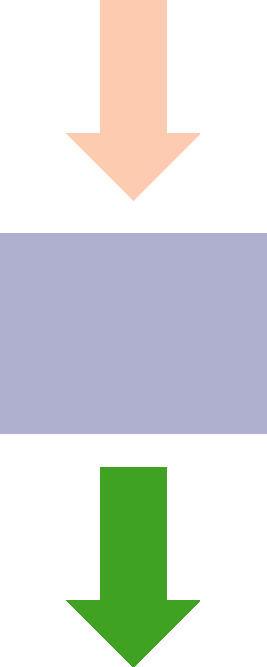
\includegraphics[width=2cm]{img/output}
	\end{column}
\end{columns}
\end{frame}
